\chapter{Struktura projektu}
\thispagestyle{chapterBeginStyle}
\label{rozdzial2}

W niniejszym rozdziale zostaną przedstawione wymagania odnośnie wymagań funkcjonalnych oraz niefunkcjonalnych implementowanej aplikacji 

\section{Wymagania niefunkcjonalne}
W niniejszej sekcji opisane zostały wymagania niefunkcjonalne dotyczące badanego algorytmu i zawierające wszystkie ograniczenia oraz zewnętrzne czynniki mające wpływ na uruchamianie lub wydajność działania programu.
\begin{enumerate}
    \item Szybkość działania programu uzależniona jest od liczby dostępnych procesorów. Jako procesor rozumie się tutaj pojedynczy wątek fizycznego procesora. Większa liczba takowych pozwala na równoległe przetwarzanie większej liczby osobników jednocześnie. Szczegóły implementacyjne zostały przedstawione w rozdziale \ref{rozdzial3}.
    \item Aplikacja jest zaprojektowana w taki sposób, aby możliwym było wygodne podmienianie jej poszczególnych modułów, które odpowiadają za jej poszczególne funkcjonalności bez potrzeby lub tylko z minimalną ingerencją w inne fragmenty kodu.
    \item Ograniczenia na rozmiar plików wczytywanych przez program oraz przez niego generowanych i zapisywanych wynikają jedynie z ograniczeń języka, w którym algorytm zaimplementowano oraz ograniczeń systemu operacyjnego, na którym program jest uruchamiany.
\end{enumerate}

\section{Wymagania funkcjonalne}
\label{sec:functional}
Poniżej zostały opisane wymagania funkcjonalne dla opisywanego algorytmu. Poniższy opis zawiera wszystkie oczekiwane cele, które powinien zrealizować program w trakcie swojego działania.

\begin{enumerate}
    \item Program wczytuje obraz, który ma zostać zreplikowany lub, w przypadku, gdy zadany plik nie istnieje, zwraca błąd i kończy działania.
    \item Program wczytuje parametry określające sposób działania algorytmu, które określają stosowaną skalę barw, liczbę iteracji algorytmu, rozmiar pojedynczego pokolenia, prawdopodobieństwo wystąpienia mutacji, dołączenie operatora krzyżowania oraz ścieżkę do pliku z obrazem, który powinien zostać zreplikowany.
    \item Parametr określający ścieżkę dostępu do pliku z obrazem replikowanym jest zawsze wymagany. Dla pozostałych parametrów program powinien przyjmować wartości domyślne, w przypadku, gdy ich wartości nie zostały zdefiniowane przy uruchomieniu programu.
    \item Parametry wywołania programu mogą również zostać podane w formie pliku konfiguracyjnego \texttt{JSON}. Ścieżka do tego pliku powinna zostać podana jako parametr wywołania programu. 
    \item Generowana jest populacja początkowa o określonej liczności i w określonej skali barw o rozdzielczości obrazu oryginalnego.
    \item Dla każdego osobnika, w każdej iteracji, stosowany jest, z określonym przez parametr wejściowy prawdopodobieństwem, operator mutacji.
    \item Każdy osobnik poddawany jest funkcji oceny i jest mu przypisywana wartość określająca jego \textit{odległość} od obrazu oryginalnego. Funkcja powinna być zaprojektowana w taki sposób, aby możliwe było sortowanie osobników względem jej wartości dla każdego z nich.
    \item Po zakończeniu każdej iteracji, o ile nie jest to ostatnia iteracja algorytmu, tworzona jest nowa populacja z osobników z bieżącego pokolenia.
    \item Jeżeli wyspecyfikowano, jest stosowany parametr krzyżowania pomiędzy dwoma osobnikami polegający na wymianie materiału genetycznego dwóch wybranych osobników z nowopowstałej populacji.
    \item Po zakończeniu działanie programu wyniki, w liczbie określonej przez jeden z parametrów wejściowych, zostają zapisane w formie plików \texttt{PNG}.
    \item Aplikacja, na etapach, które umożliwiają zastosowanie takiego rozwiązania, powinna wykonywać swoje obliczenia równolegle. Powinna zostać zapewniona odpowiednia synchronizacja pomiędzy poszczególnymi wątkami.
\end{enumerate}

\section{Diagram przepływu}
\label{sec:flowchart_desc}
Na grafice \ref{fig:flowchart} przedstawiono diagram przepływu dla projektowanej aplikacji. Diagram ten przedstawia poszczególne zadania wykonywane przez program, które zostały zawarte w wymaganiach funkcjonalnych opisanych w podrozdziale \ref{sec:functional}.

Program rozpoczyna swoje działanie od wczytania wymaganych danych. Następnie zostaje zainicjalizowane pierwsze pokolenie, które będzie przetwarzana w pierwszej iteracji algorytmu. Następnie na każdym osobników zostaje zastosowany operator mutacji, a następnie każdy z nich zostaje poddany funkcji oceny. Ten etap został urównoleglony, co zostało zaznaczone na diagramie. Następnie osobniki są sortowane względem wartości funkcji celu i wybierane są osobniki, które utworzą następne pokolenie - $k$ najlepszych osobników, czyli takich, dla których funkcja celu przyjęła wartości najmniejsze. Parametr $k$ jest ustawiany przez jeden z parametrów wejściowych. Następnie najlepsze osobniki są kopiowane w taki sposób, aby liczność nowego pokolenia była zgodna z wartością podaną przez użytkownika w postaci parametru. Ta część działania programu również jest wykonywana współbieżnie. Po tym etapie, w przypadku gdy operator krzyżowania został dozwolony przez użytkownika, następuje krzyżowanie osobników (ten etap również jest wykonywany równolegle), a w przeciwnym wypadku program przechodzi do kolejnej iteracji. Po czasie, gdy program osiągnie zadaną liczbę iteracji, zostaje wybranych $k$ najlepszych obrazów z ostatniego pokolenia i zostają one zapisane w formie plików \texttt{PNG}. Po wykonaniu tej operacji program kończy działanie. Szczegóły dotyczące implementacji zostały przedstawione w rozdziale \ref{rozdzial3}.

\begin{figure}
    \centering
    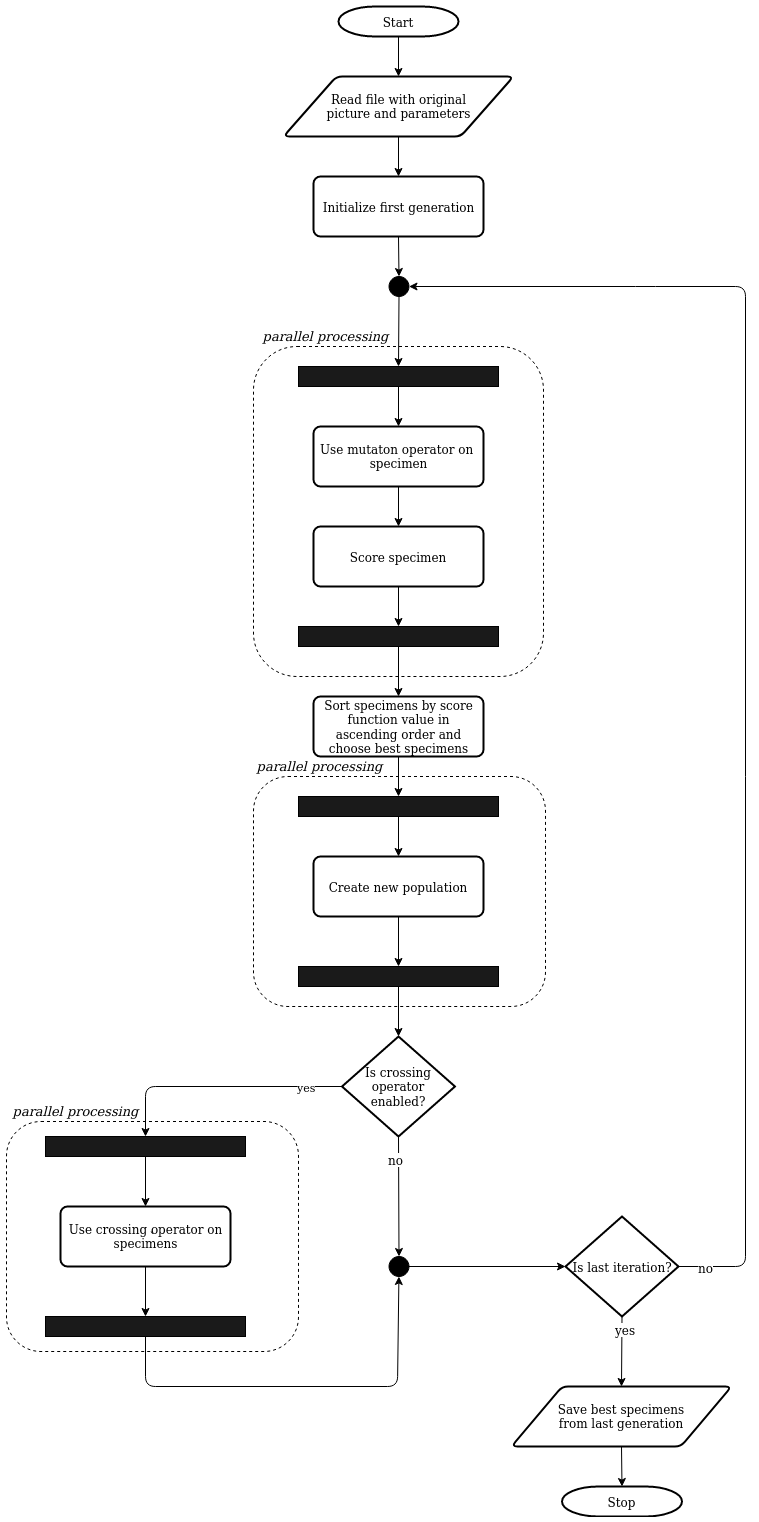
\includegraphics[scale=0.38]{images/other/thesis_flowchart.png}
    \caption{Diagram przepływu dla aplikacji. Program, po rozpoczęciu działania wczytuje odpowiednie pliki i parametry konfiguracyjne oraz inicjalizuje pierwsze pokolenie. Następnie stosowane są operator mutacji oraz funkcja oceny. Dalej tworzona jest nowa populacja i, jeżeli konfiguracja to przewiduje, stosowany jest operator krzyżowania. Program kończy działanie po określonej liczbie iteracji i zapisuje wyniki do odpowiednich plików po czym kończy działanie. Części algorytmu, które zostały urównoleglone zostały odpowiednio opisane na diagramie. Szczegółowy jego opis znajduje się w rozdziale \ref{sec:flowchart_desc}.}
    \label{fig:flowchart}
\end{figure}

\section{Komponenty aplikacji}
\label{sec:components_desc}
Prezentowana w pracy aplikacja składa się z różnych komponentów, gdzie każdy z nich spełnia określoną funkcjonalność niezbędną dla poprawnego działania aplikacji. W prezentowanej implementacji można wyróżnić następujące komponenty, które zostały przedstawione również na diagramie \ref{fig:components_chart}.

\subsection{Moduł konfiguracji}
\label{subsec:configuration_module}
Moduł odpowiedzialny za konfigurację algorytmu wczytuje parametry, które pozwalają na zdefiniowanie sposobu działania programu i przetrzymuje je w pamięci operacyjnej w taki sposób, aby były one dostępne dla pozostałych modułów aplikacji. 

\subsection{Moduł obsługi wejścia/wyjścia}
\label{subsec:io_module}
Moduł jest odpowiedzialny za wczytywanie plików (obraz, który ma zostać zreplikowany) oraz zapisanie rozwiązań wygenerowanych przez program po ostatniej iteracji algorytmu. Moduł obsługuje i wyświetla błędy związane z obsługą plików.

\subsection{Moduł genetyki}
\label{subsec:genetics_module}
Moduł obsługuje i definiuje działanie operatorów genetycznych (mutacji i krzyżowania) oraz odpowiada za wyliczanie funkcji celu dla każdego osobnika. Moduł ten jest \textit{wymienny} i może zostać przedefiniowany przez użytkownika przy warunku spełniania zadanego przez autora interfejsu.

\subsection{Moduł funkcji pomocniczych}
\label{subsec:helpers_module}
Komponent zawierający funkcje pomocnicze służące, między innymi, do sortowania osobników względem podanej wartości (w tym przypadku - względem funkcji celu), wyliczania wartości koloru dla pikseli dla operator mutacji, wyliczania wartości pomocniczych dla modułu genetyki. Szczegółowa specyfikacja tego modułu jest zawarta w dokumentacji technicznej kodu.

\subsection{Moduł obsługi współbieżności}
\label{subsec:threading_module}
Moduł odpowiedzialny za obsługę zadań, które mogą zostać obsłużone współbieżnie. Zostały one wyszczególnione na diagramie \ref{fig:flowchart}. Jego zadaniem jest rozdzielenie zadań pomiędzy poszczególne wątki oraz synchronizacja momentu ich zakończenia.

\begin{figure}
    \centering
    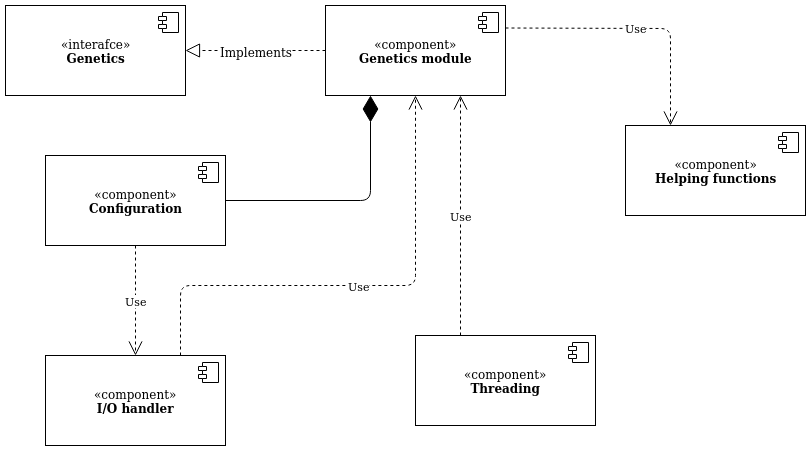
\includegraphics[scale=0.5]{images/other/components.png}
    \caption{Diagram komponentów aplikacji. Każdy z widocznych na grafice komponentów spełnia odpowiednią funkcjonalność, gdzie każdy z nich został krótko opisany w odpowiednim podrozdziale: interfejs \textit{Genetics} oraz komponent \textit{Genetics module} odpowiedzialne za logikę genetyki algorytmu opisane są w podrozdziale \ref{subsec:genetics_module}; \textit{Helping funcions} zawierajacy metody pomocnicze dla modułu genetyki opisany jest w podrozdziale \ref{subsec:helpers_module}; \textit{Configuration} odpowiedzialny za przechowywanie zdefiniowanej przez użytkownika konfiguracji algorytmu opisany jest w podrozdziale \ref{subsec:configuration_module}; \textit{Threading} odpowiedzialny za obsługę współbieżności w aplikacji opisany jest w sekcji \ref{subsec:threading_module}; moduł \textit{I/O handler} odpowiedzialny za obsługę wczytywanych i zapisywanych plików opisany jest w podrozdziale \ref{subsec:io_module}.
    }
    \label{fig:components_chart}
\end{figure}
